%!TeX ts-program = xelatex
%!TeX encoding = utf-8 Unicode
\documentclass[11pt,a4paper]{article}
\usepackage{listings}

\usepackage{color}
\usepackage{graphics}
\definecolor{dkgreen}{rgb}{0,0.6,0}
\definecolor{gray}{rgb}{0.5,0.5,0.5}
\definecolor{mauve}{rgb}{0.58,0,0.82}

\lstset{frame=tb,
	language=Python,
	aboveskip=3mm,
	belowskip=3mm,
	showstringspaces=false,
	columns=flexible,
	basicstyle={\small\ttfamily},
	numbers=none,
	numberstyle=\tiny\color{gray},
	keywordstyle=\color{blue},
	commentstyle=\color{dkgreen},
	stringstyle=\color{mauve},
	breaklines=true,
	breakatwhitespace=true,
	tabsize=3
}
\usepackage[margin=0.5in]{geometry}
\title{Assignment on Quality (based on Lecture 4)}
\author{Vishal M Kalathil}

\begin{document}

\maketitle
\section{Composite Time Domain Signal} % (fold)
	\subsection{Code} % (fold)
	    \lstinputlisting[language=Python]{sine_waves.py}  
	    \newpage
	\subsection{Graph}%
	     \begin{figure}[hb]
	          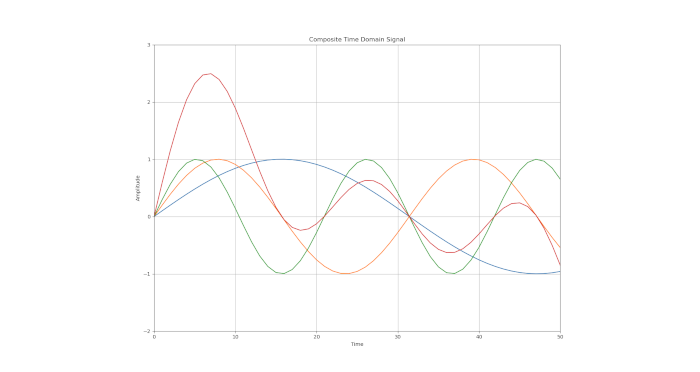
\includegraphics{sine_waves.png}
	          \caption{The red line is the composite time domain signal}
	      \end{figure}
	      \newpage
\section{SawTooth} % (fold)
	\subsection{Code} % (fold)
	      \lstinputlisting[language=Python]{sawtooth.py} 
	\subsection{Graph}%
	     \begin{figure}[hb]
	          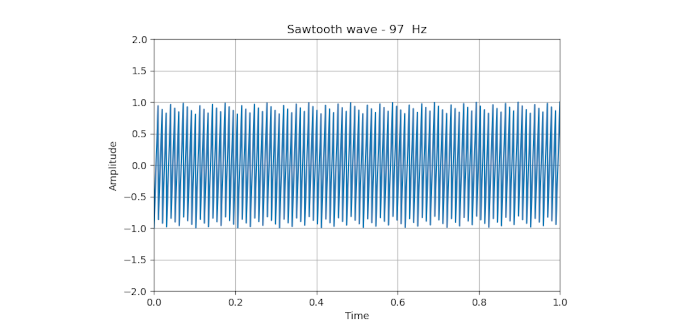
\includegraphics{sawtooth.png}
	      \end{figure} 
	      \newpage
\section{Triangle} % (fold)
	\subsection{Code} % (fold)
	      \lstinputlisting[language=Python]{triangle.py}  
	\subsection{Graph}%
	     \begin{figure}[hb]
	          \includegraphics{Triangle.png}
	      \end{figure} 
	      \newpage
\section{Square} % (fold)
	\subsection{Code} % (fold)
	      \lstinputlisting[language=Python]{square.py}  
	\subsection{Graph}%
	     \begin{figure}[hb]
	          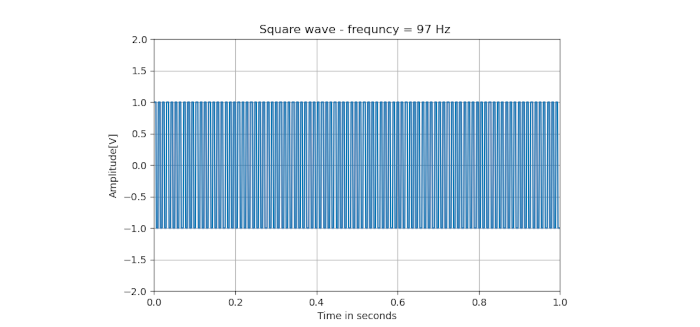
\includegraphics{square.png}
	      \end{figure}
	      \newpage
\section{Fourier's Transformation} % (fold)
	Fourier analysis is a method for expressing a function as a sum of periodic components, and for recovering the signal from those components. 
	When both the function and its Fourier transform are replaced with discretized counterparts, it is called the discrete Fourier transform (DFT).
	\newline
	\begin{enumerate}
	    \item In python we can use scipy fft or numpy fft to analyze the Fourier
	        Transformation
	    \item In MATLAB we use fft to do the same
	  \end{enumerate}
\end{document}
